\documentclass[]{article}
\usepackage{graphicx}
\usepackage{amsmath}
\usepackage{amssymb}
\usepackage{amsfonts}
\usepackage{fancyhdr}
\usepackage[headheight=65pt,tmargin=150pt,headsep=95pt]{geometry}
\usepackage{ragged2e}
\usepackage{array}
\usepackage{tabularx}



\graphicspath{{./images/}}

\pagestyle{myheadings}
\markright{Binary black hole detections\hfill 2663452m\hfill 12/04/2023\hfill}

\title{\textbf{Binary black hole detections from LIGO-VIRGO runs 1 and 2}}
\author{2663452m (University of Glasgow)}
\date{12/04/2023}



\begin{document}
\maketitle

\begin{abstract}

\end{abstract}
\twocolumn
\newpage





\section*{Introduction and Background}
Gravitational waves as first predicted by Albert Einstein in 1915 in his paper on
special and general relativity, are ripples in the fabric of space-time due to the acceleration of large masses
and have been notoriously hard to detect. That was until
the LIGO Michelson interferometer in Hanford and Livingston was complete in 2015.
A Michelson interferometer is a device that uses the interference of two beams of
light to detect small changes in the path distance of the two beams. A diagram of one can
be seen in Figure 1.
\begin{figure}[h]
    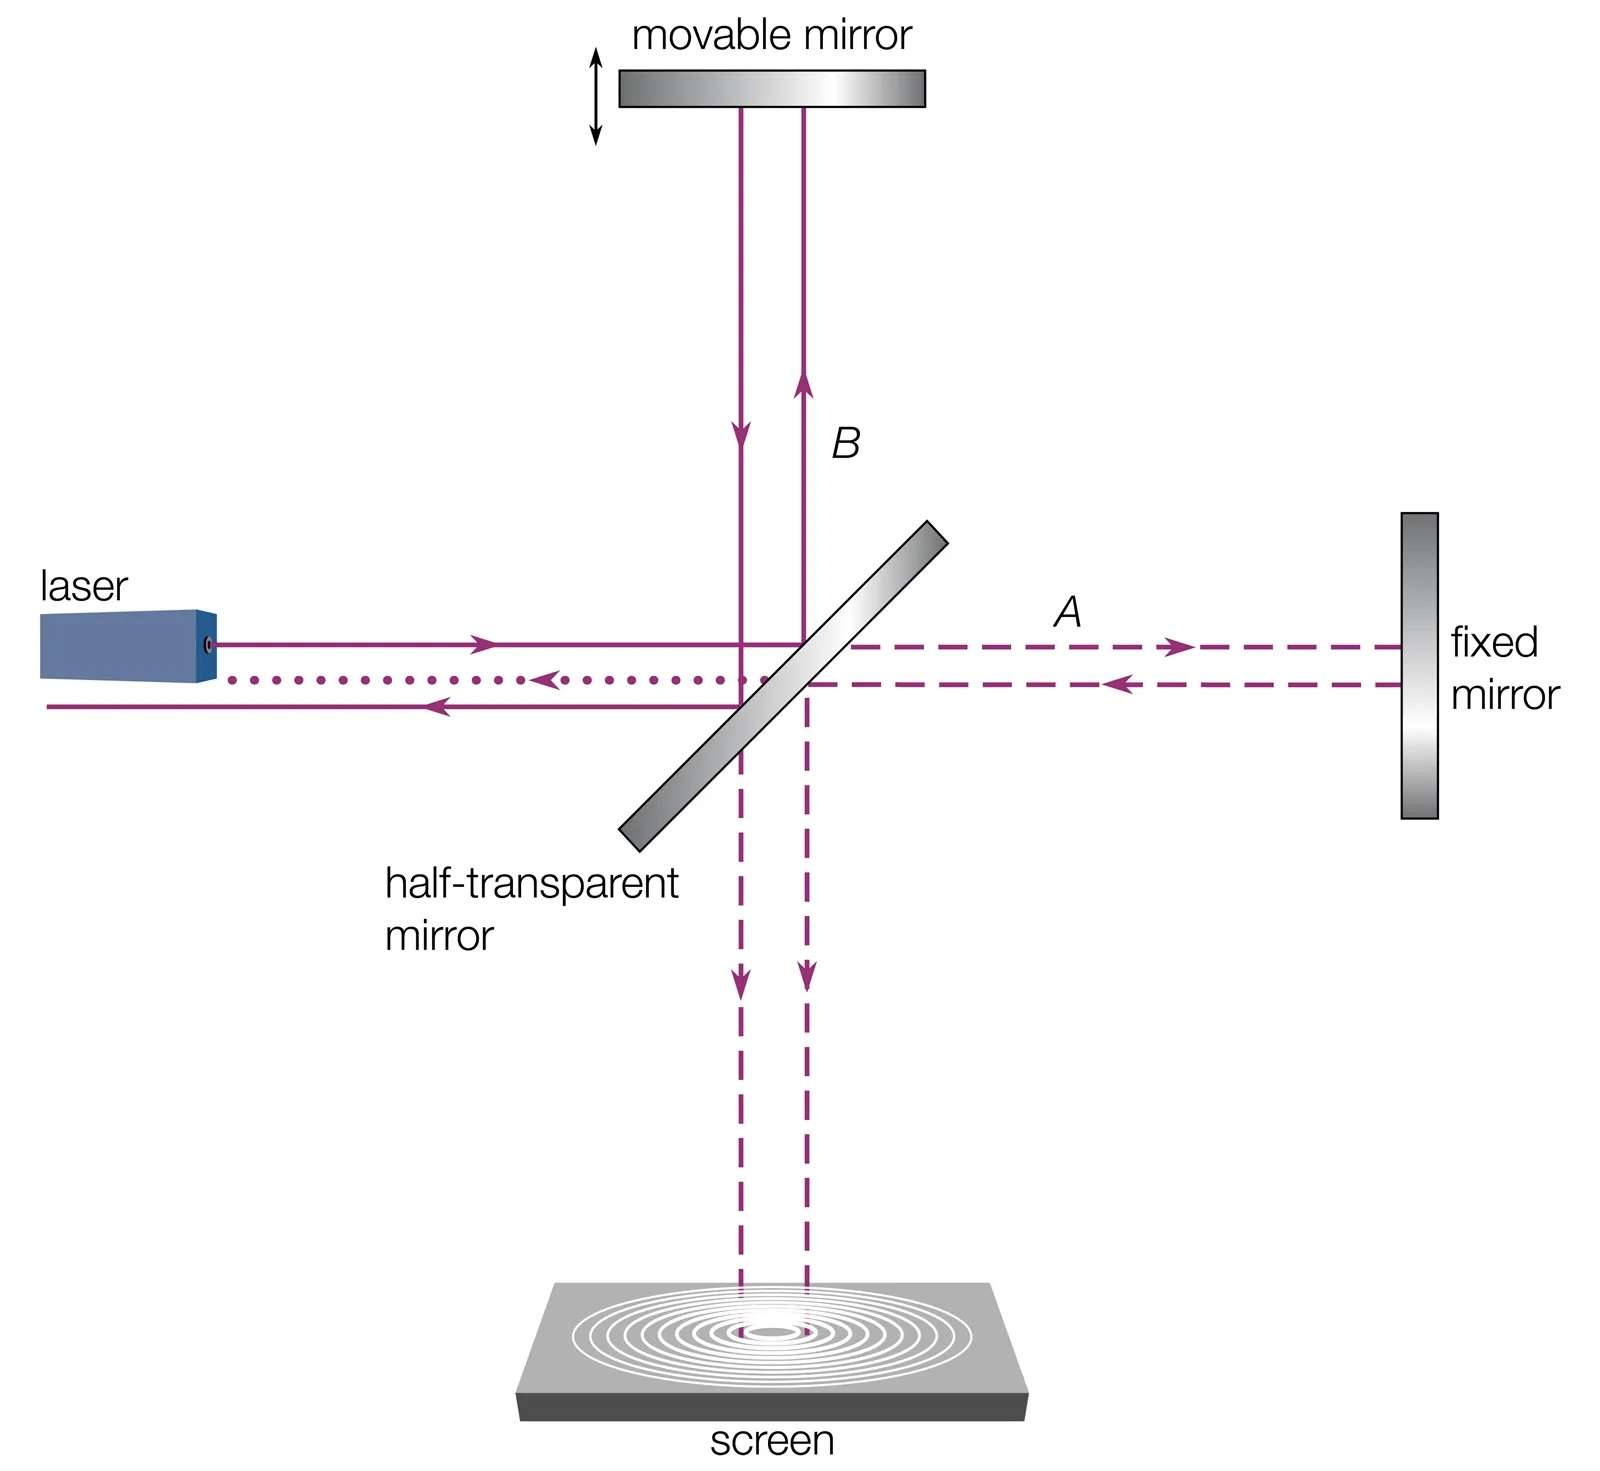
\includegraphics[width=6cm]{images/michelson_interferometer.png}
    \caption{Diagram of a michelson interferometer as used in LIGO.$^1$}
    \label{fig:michelson}
    \end{figure}
By using a Michelson interfermoeter in the LIGO experiment the small changes in
distance that are required can be detected and measured. These distances can be on the
order of 10$^{-21}$m this distance is calle dthe strain of the wave and
is the amount of stretching over the original length and can be approximated as
\begin{equation}h \approx \frac{GM}{c^2d}\left(\frac{v}{c}\right)^2 \label{eq:strain}\end{equation}
where $G$ is the gravitational constant, $M$ is the mass of the source, $c$ is the speed of light,
d is the distance to the source and $v$ is the velocity of the system.

caused by the passing of gravitational waves moving at the speed of light
through the
interferometer arms (which results in a shift in the interference pattern of the light beams).
The first detection of a gravitational wave was on the 14th of
September 2015, just 100 years after the publication of Einstiens paper.
The first detection was of a binary black hole merger, these mergers commonly
release a large amount of energy in the form of gravitational waves. This happens
because as the two black holes accelerate towards each other they warp the
space-time around them, and as they approach the point of coalescence the amplitude
of these waves massively increases, thus allowing them to be detected over the Background
noise. The run-down after merging is extremely quick and thus leaving a distinct peak
at the time of coalescence. In this report the first 11 detections of gravitational waves
as a result of binary black hole mergers will be analysed and discussed. Starting with GW150914.

\section*{GW150914}
To be able to carry out the analysis of the gravitaional waves it was necessary to set
up our workspace to be able to use some provided function and packages written by the
LIGO collaboration. This was done by first installing the LIGO lalsuite package for Python 3.10
and then importing the packages into our notebook. The package contains a number of useful
functions that will be discussed in more detail later in this report.
For the first detection of gravitational waves GW150914 the data was provided
by the university through the Jupyter Hub. Once this data was loaded in
the first step was to plot the strain against the time and identify by eye the peak
of the gravitational wave. This plot is shown in Figure 2.
\begin{figure}
    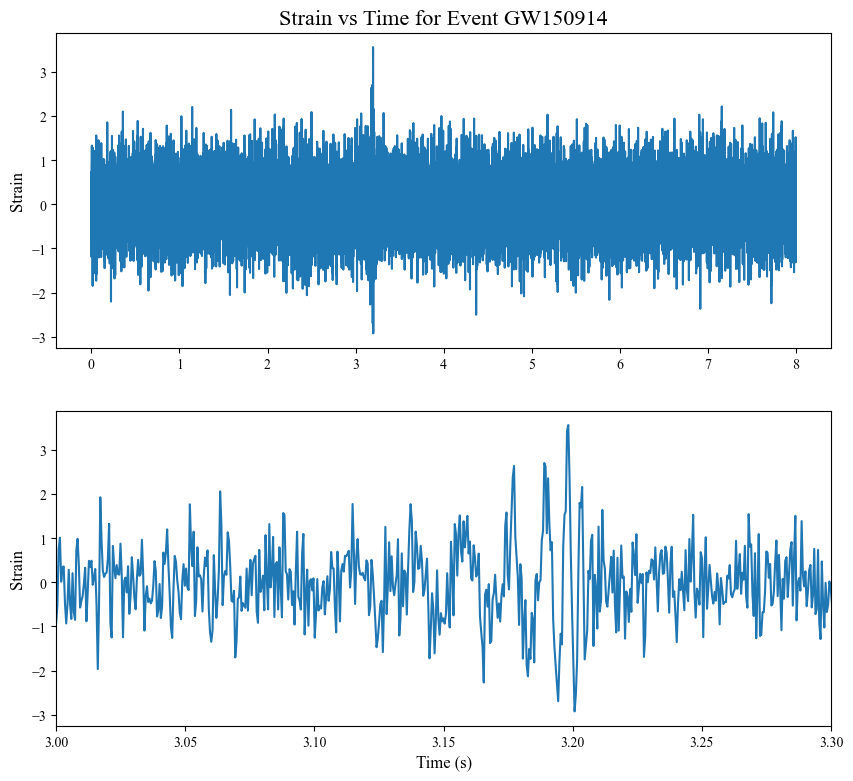
\includegraphics[width=6cm]{images/Signal_gw150914.png}
    \caption{top: Plot of the strain against time for GW150914 bottom:
    limited to shorter time to resolve the peak more.}
    \label{fig:GW150914}
\end{figure}
\newpage
From Figure 2 it can be seen that the peak of the gravitaional wave occurs at
around 3.2 seconds.
Knowing this time we can use the SCIPY package to generate a spectrogram of strain and frequency and from this a color plot can be
created which visualizes the amount of energy in the gravitational wave at a given
frequency and time. This plot is shown in Figure 3.
\begin{figure}[h]
    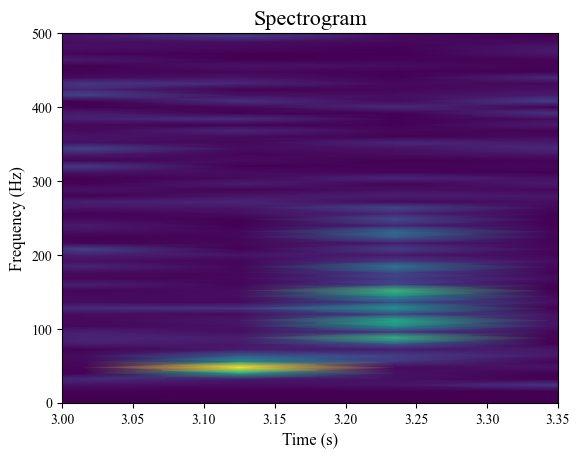
\includegraphics[width=6cm]{images/spectrogram_gw150914.png}
    \caption{Spectrogram of GW150914, showing the 'chirp' track of the gravitational wave.}
    \label{fig:spectrogram}
\end{figure}
\newline
In this plot the point where the energy is high across multiple frequencies
correlates with the same time as the peak in the strain in Figure 2.

Now that we have visualised the actual data form the gravitational wave, it would now
be useful to be able to compare this to the theorectical prediction of the event.
This can be generated using the make template function as supplied by the LIGO
collaboration. This function takes in the masses of the two black holes and
the time, frequency, distance and uncertainty on the data. The function then returns
a strain and time array that can be used to plot the theorectical predictions.
This produces an ideal signal as seen in Figure 4, this is easier to see the signal as,
it no longer has any noise.
\begin{figure}[h]
    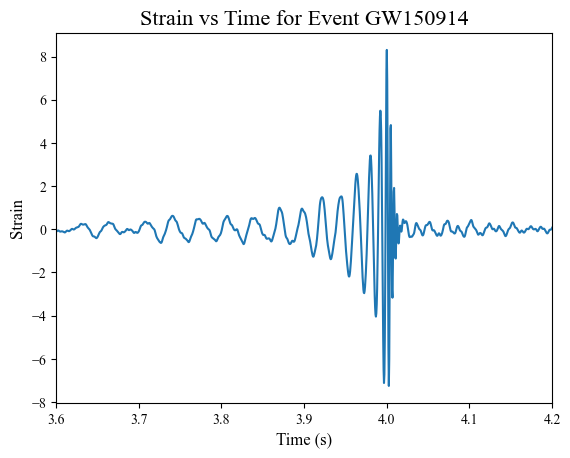
\includegraphics[width=6cm]{images/ideal_signal_gw150914.png}
    \caption{Theoretical prediction for GW150914}
    \label{fig:ideal_signal}
\end{figure}
\newline
Later this template will be overlayed on the true data to determine the goodness of fit.
\section*{Detecting the signals for the ten Black hole Mergers}
To determine the signal of the data for the ten black hole mergers the signal
to noise ratio was used to determine the strength of the signal and its location in time.
This could be done using the function given in the lalsuite package. This function
returns a list of signal to noise ratios for each time in the data. If the SNR is low then the
template that was put into the function is badly aligned or the masses of the black holes
that were put into the template function are incorrect, and if the SNR is high
then the template is aligned well and the masses are correct. An example SNR time series
is shown in Figure 5.
\begin{figure}[h]
    \includegraphics[width=6cm]{images/SNR_gw150914.png}
    \caption{SNR time series for GW150914, with the peak at 3.2 seconds which tells
    us it is correctly aligned as this is the same time as obtained above}
    \label{fig:SNR}
\end{figure}
This SNR at the peak is important as it can be used later to determine the masses of the
black holes as well as other important information. So this value was stored to be used later.

\section*{Determining the masses of the black holes}
To determine the masses of the black hole pairs, some assumptions were made
about the system. The first assumption was that m1 the mass of the first black hole is larger
than m2 the mass of the second black hole. And the second assumption was that m1/m2 is less than 8
as this is the maximum mass ratio expected and it helps lower the number of possible mass pairs
for the next section. With these assumptions the mass of the black holes can be determined using
nested for loops to iterate over 10,000 possible mass pairs and calculate the SNR for each pair, then storing this
SNR and the corresponding mass pair. This was done for the 10 binary black hole mergers (the binary neutron star
merger was not included in this section as it has different mass ranges, and thus will be analysed seperately
later). With the SNR's and the mass pair options stored a color plot was created for each event, where
the intensity of the color is proportional to the SNR and the x and y axis are the mass of each black hole.
An example of one of these plots is shown in Figure 6.
\begin{figure}[h]
    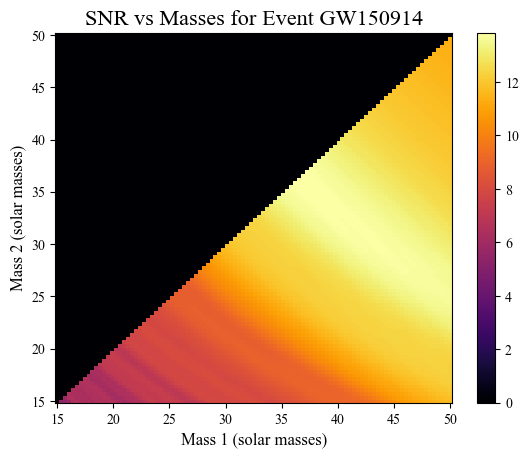
\includegraphics[width=6cm]{images/snr_color.png}
    \caption{Mass plot for GW150914, showing the mass pairs that give the highest SNR}
    \label{fig:mass_plot}
\end{figure}
\newline
The black upper triangle is due to the conditional statement that mass one must be greater than mass two. Where the
color is the highest is where the SNR is highest and thus the mass pair that is most likely
to be correct. From this plot and as discussed above the mass pair that is most likely to
be correct is 36.06 ± 1.4 and 35.74 ± 4.3 solar masses. This is within estimated error of to the masses published
by the LIGO collaboration of 35.6 and 30.6 solar masses

\section*{Determining estimates for the distance, time and phase of coalescence}

\begin{table*}[t]
    \begin{center}
        \begin{tabular}{|c c c c c c|}
            \hline
            Event & Distance (Mpc) & Time (s) & Phase (rad) & Mass one ($M_{\odot}$) & Mass two ($M_{\odot}$)\\
            \hline
            GW150914 & 1128 $\pm$ 82 & 3.198 $\pm$ 0.000 & 0.03 $\pm$ 0.16 & 36.06 & 35.76 \\
            GW151012 & 3783 $\pm$ 1677 & 2.703 $\pm$ 0.001 & 0.00 $\pm$ 0.82 & 35.40 & 11.72 \\
            GW151226 & 1812 $\pm$ 552 & 2.067 $\pm$ 0.000 & 0.00 $\pm$ 0.46 & 12.10 & 9.70 \\
            GW170104 & 2119 $\pm$ 340 & 1.975 $\pm$ 0.000 & 1.79 $\pm$ 0.32 & 35.86 & 25.35 \\
            GW170608 & 664 $\pm$ 81 & 3.794 $\pm$ 0.000 & 2.67 $\pm$ 0.18 & 11.27 & 8.36 \\
            GW170729 & 3150 $\pm$ 590 & 3.539 $\pm$ 0.001 & 2.89 $\pm$ 0.51 & 75.15 & 29.70 \\
            GW170809 & 2146 $\pm$ 444 & 2.641 $\pm$ 0.001 & 2.78 $\pm$ 0.42 & 46.41 & 15.10 \\
            GW170814 & 2268 $\pm$ 385 & 3.335 $\pm$ 0.000 & 0.00 $\pm$ 0.34 & 30.20 & 29.85 \\
            GW170818 & 1596 $\pm$ 417 & 2.161 $\pm$ 0.000 & 0.73 $\pm$ 0.40 & 12.79 & 9.91 \\
            GW170823 & 4111 $\pm$ 1121 & 4.456 $\pm$ 0.001 & 0.00 $\pm$ 0.64 & 55.25 & 26.26 \\
            \hline
        \end{tabular}
        \caption{Estimated values for the distance, time and phase of coalescence and the mass pairs for the ten binary black hole mergers}
        \label{tab:estimates}
    \end{center}
\end{table*}

To find estimates for the distance, time and phase of coalescence the make template function was used again
to generate a template for each event but this time using the masses as found above,
as this would produce the most accurate templates for the sets of data.
From this the SCIPY curve fit function could be used as this allow for estimated of unknown quantities depending on the
how close the tru data/plot is to the template. However for this particlar application
it was necessary to provide some upper and lower bounds that these value could take as this reduces the possible sollutions
to the problem. These bounds were determined by looking at the peak and its location as well as an overall generic distance range
for the events. The curve fit function also provides a covariance matrix which can be used to determine the error on the
estimated values. This was repeated for each event and the results are shown in Table 1.




\section*{Analysis}

\section*{Conclusion}

\section*{References}
\end{document}
